\documentclass[pdftex,12pt,xcolor=svgnames]{beamer}

\mode<presentation>
{
  \usetheme{boxes}
  \usecolortheme[named=MidnightBlue]{structure}
  %\setbeamercolor{normal text}{bg=NavajoWhite!20}
  %% \usefonttheme{serif}
  \setbeamertemplate{navigation symbols}{}
  % Show frame number and author name in footline
  \setbeamertemplate{frametitle}[default][center]
  \setbeamertemplate{footline}[frame number]
  \setbeamertemplate{items}[circle]
  %\addtobeamertemplate{footline}{\quad\textcolor{gray}{James Robert Lloyd}}{}
  % Set frame titles in small capitals
  %% \setbeamerfont{frametitle}{shape=\scshape,family=\rmfamily,size={\fontsize{16}{20}}}
  %% \setbeamercolor{frametitle}{bg=gray!60!white,fg=black}
  %% \setbeamercolor{frametitle}{bg=blue,fg=black}
  % Alerted text: blue (uncomment second line if theme sets alerted text to bold)
  \setbeamercolor{alerted text}{fg=blue}
  %\setbeamerfont*{alerted text}{}
  \setbeamertemplate{bibliography item}[text] %{\hbox{\donotcoloroutermaths$\blacktriangleright$}}
  \setbeamertemplate{bibliography entry title}{}
  \setbeamertemplate{bibliography entry author}{}
  \setbeamertemplate{bibliography entry note}{}
  \setbeamertemplate{bibliography entry location}{}

}
\usepackage[english]{babel}
\usepackage[latin1]{inputenc}
\usepackage{times}
\usepackage[T1]{fontenc}
\usepackage{hyperref}
\usepackage{multimedia}
\usepackage{eepic}
\usepackage{graphicx}
%\usepackage[nohug]{latexinclude/diagrams}
\usepackage{tikz}
\usetikzlibrary{calc}

%% \newcommand{\footlineextra}[1]{
%%     \begin{tikzpicture}[remember picture,overlay]
%%         \node[yshift=1.5ex,anchor=south east] at (current page.south east)
%% {#1};
%%     \end{tikzpicture}
%% }

\newcommand{\footlineextra}[1]{
    \begin{tikzpicture}[remember picture,overlay]
        \node[xshift=-5ex,yshift=-0.5ex,anchor=south east] at (current page.south east)
             {\mbox{\tiny \textcolor{MidnightBlue}{#1}}};
    \end{tikzpicture}
}

\def\sectionframe#1{
  {
    \setbeamertemplate{footline}{\empty}
    \begin{frame}{}
      \begin{center}
        \huge\sc #1
      \end{center}
    \end{frame}
  }
}


\usepackage{etex}
\usepackage{tabularx}
\usepackage{include/picins}
\usepackage{include/preamble}
\usepackage{setspace}
\usepackage{xcolor}
\usepackage{tikz}
\usepackage{listings}
%\usepackage{algorithm}
%\usepackage{algpseudocode}

\definecolor{Blue}{rgb}{0.0,0.0,1.0}
\lstloadlanguages{Python}%
\lstset{language=Python,
        frame=none,
        basicstyle=\tiny\ttfamily\bfseries,
        keywordstyle=[1]\color{Blue},
        keywordstyle=[2]\color{Purple},
        commentstyle=\usefont{T1}{pcr}{m}{sl}\color{Green},
        keepspaces=true,
        }
\lstset{language=Python} 

%%%%%%%%%%%%%%%%%%%%%%%%%%%%%%%%%%%%%%%%%%%
%
% Some look and feel definitions
%
%%%%%%%%%%%%%%%%%%%%%%%%%%%%%%%%%%%%%%%%%%%

\setlength{\columnsep}{0.03\textwidth}
\setlength{\columnseprule}{0.0018\textwidth}
\setlength{\parindent}{0.0cm}
\hypersetup{colorlinks=true,citecolor=blue}
\newcommand{\paren}[1]{\left( #1 \right)}
\newcommand{\vv}{\mathbf{v}}
%%%%%%%%%%%%%%%%%%%%%%%%%%%%%%%%%%%%%%%%%%%
%
% The talk
%
%%%%%%%%%%%%%%%%%%%%%%%%%%%%%%%%%%%%%%%%%%%

\title{Meta-learning: why not use gradients?}

\author{
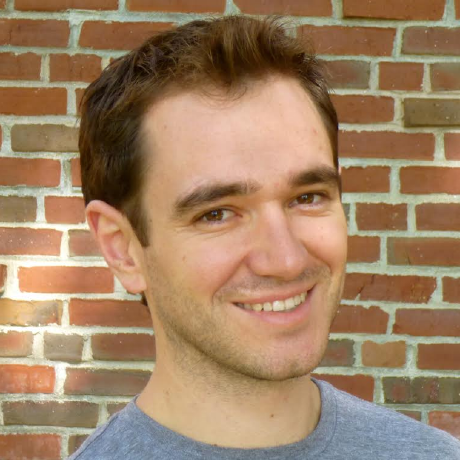
\includegraphics[height=0.16\textwidth]{talkfigs/dougal}
\qquad\qquad
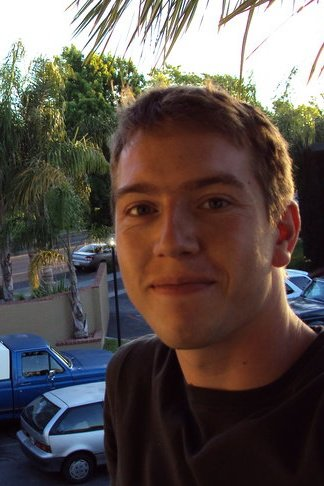
\includegraphics[height=0.16\textwidth, trim=20mm 25mm 0mm 25mm, clip]{talkfigs/david2}
\qquad\qquad
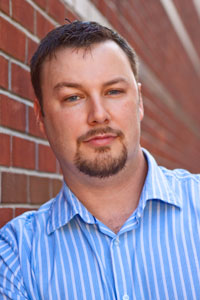
\includegraphics[height=0.16\textwidth]{talkfigs/adams}
\\
Dougal Maclaurin, David Duvenaud, Ryan Adams}

\institute{Harvard University}

\begin{document}

\frame[plain] {\titlepage}

\frame[plain]{
\frametitle{Motivation}
\begin{itemize} 
  \item Hyperparameters are everywhere
  \item Gradient-free optimization fails in high dimensions
  \item Validation loss is a just a function
  \item Why not take gradients?
\end{itemize}}

\frame[plain]{\frametitle{Reverse-mode Differentiation}
\begin{align*}
\onslide<1->{\pderiv{}{x} L\paren{F\paren{G\paren{H\paren{x}}}}
             & = \pderiv{L}{F}\pderiv{F}{G}\pderiv{G}{H}\pderiv{H}{x} \\}
\onslide<2->{& = \pderiv{L}{F}\paren{\pderiv{F}{G}\paren{\pderiv{G}{H}\pderiv{H}{x}}} \quad &\text{Forward mode}\\
             & = \paren{\paren{\pderiv{L}{F}\pderiv{F}{G}}\pderiv{G}{H}}\pderiv{H}{x} \quad &\text{Reverse mode}}
\end{align*}
\onslide<3>{
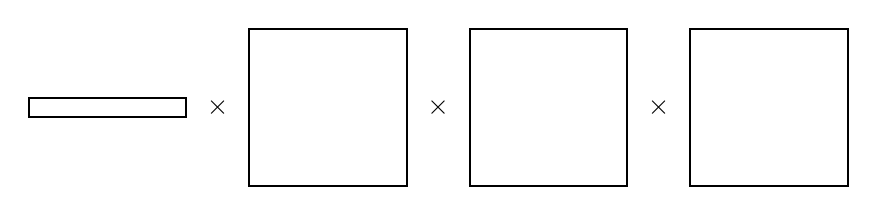
\begin{tikzpicture}[thick, scale=0.4]
  \draw (1,3.2) rectangle (6, 3.8);
  \draw (8,1) rectangle (13, 6);
  \draw (15,1) rectangle (20, 6);
  \draw (22,1) rectangle (27, 6);
  \node at (7, 3.5) {$\times$};
  \node at (14, 3.5) {$\times$};
  \node at (21, 3.5) {$\times$};
\end{tikzpicture}}
}

\frame[plain]{\frametitle{FunkyYak: Automatic Differentiation} 
\begin{itemize} 
  \item \url{github.com/HIPS/FunkyYak}
  \item Simple ($\sim$ 300 lines of code)
  \item Functional interface
  \item Works with (almost) arbitrary Python/numpy code
  \item Can take gradients all the way down
  \item The second most popular automatic differentiation package written at Harvard in fall 2014
\end{itemize}}

\frame[plain]{\frametitle{FunkyYak Examples}
\begin{columns}
\begin{column}{5.5cm}
\lstinputlisting{code/sinusoid.py} 
\end{column}
\begin{column}{5cm}
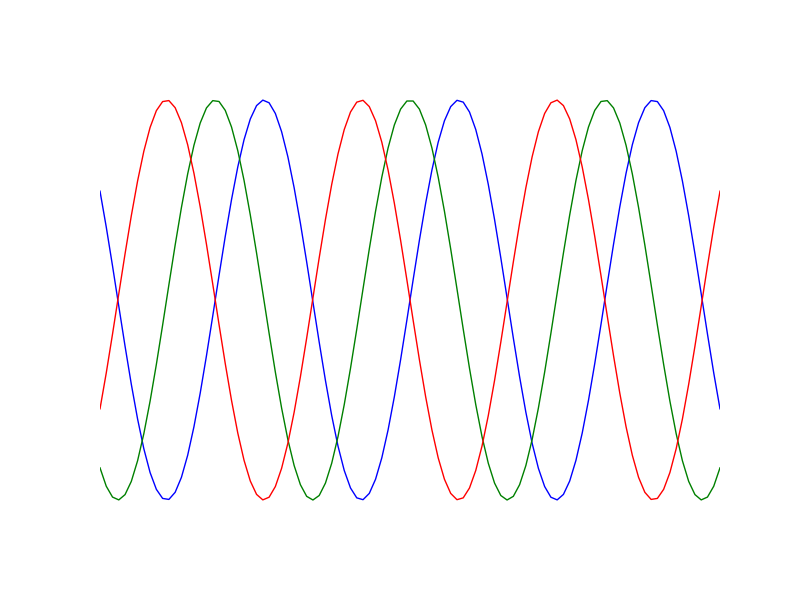
\includegraphics[width=6cm]{code/sinusoid.png}
\end{column}
\end{columns}}

\frame[plain]{\frametitle{FunkyYak Examples}
\begin{columns}
\begin{column}{5.5cm}
\lstinputlisting{code/sinusoid-taylor.py} 
\end{column}
\begin{column}{5cm}
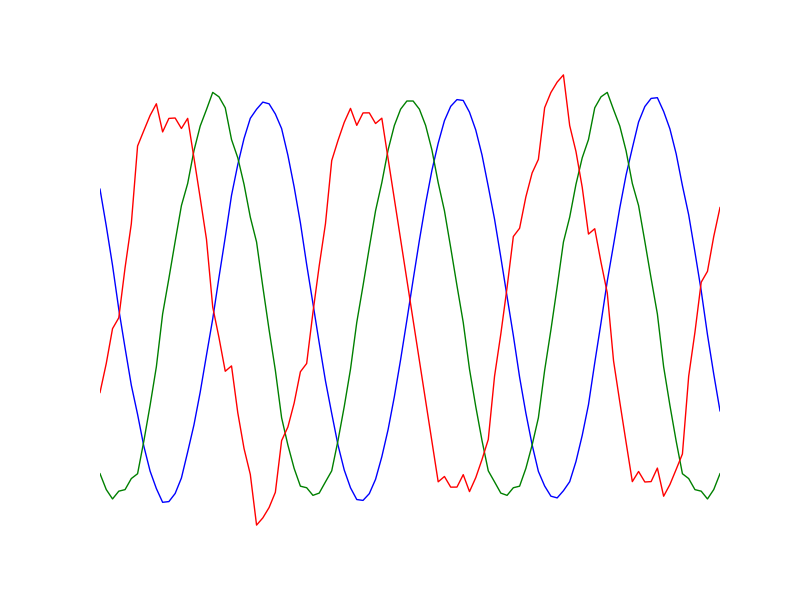
\includegraphics[width=6cm]{code/sinusoid_taylor.png}
\end{column}
\end{columns}}

\frame[plain]{\frametitle{FunkyYak Examples}
\begin{columns}
\begin{column}{5.5cm}
\lstinputlisting{code/tanh.py}
\end{column}
\begin{column}{5cm}
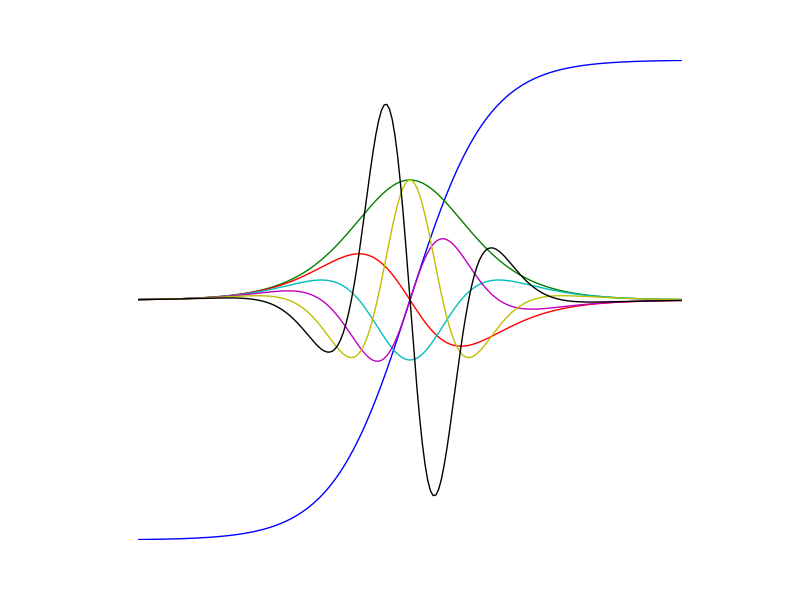
\includegraphics[width=6cm]{code/tanh.png}
\end{column}
\end{columns}}

\frame[plain]{\frametitle{SGD is just a function}
\includegraphics<1>[width=0.9\columnwidth]{talkfigs/learning_curves_1.pdf}
\includegraphics<2>[width=0.9\columnwidth]{talkfigs/learning_curves_2.pdf}
\includegraphics<3>[width=0.9\columnwidth]{talkfigs/learning_curves_3.pdf}}

\frame[plain]{\frametitle{Example uses of hyper-gradients: learning rates}
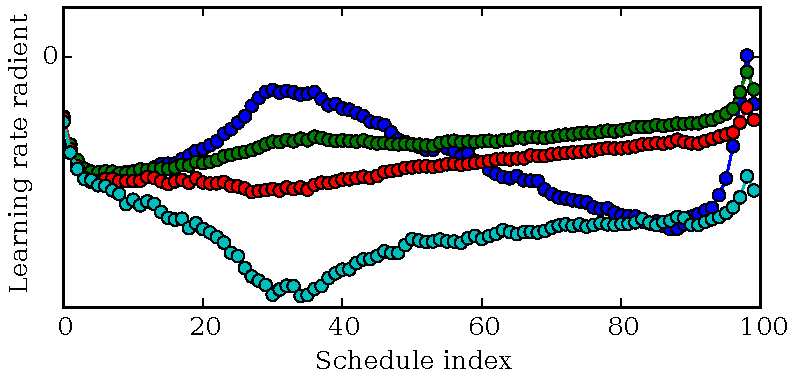
\includegraphics[width=\columnwidth]{../experiments/Feb_3_training_schedules/5_initial_gradient/schedules_small.pdf}}

\frame[plain]{\frametitle{Example uses of hyper-gradients: learning rates}
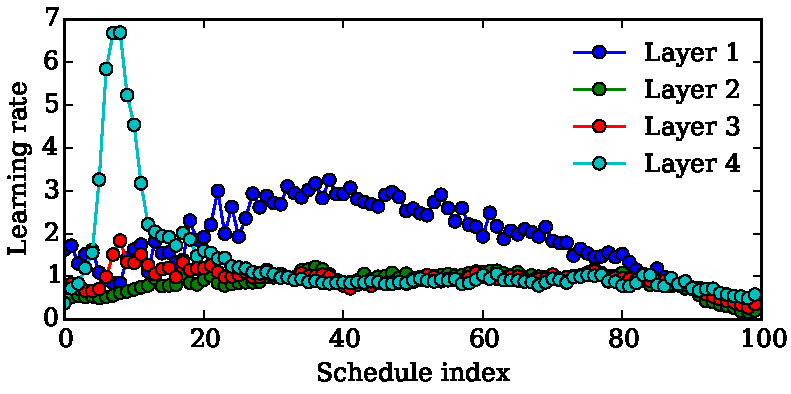
\includegraphics[width=\columnwidth]{../experiments/Feb_3_training_schedules/3_adam_50/schedules_small.pdf}}

\frame[plain]{\frametitle{Optimizing initialization distributions} 
\begin{center}
\begin{tabular}{cc}
 Biases & Weights \\
\hspace{-1em}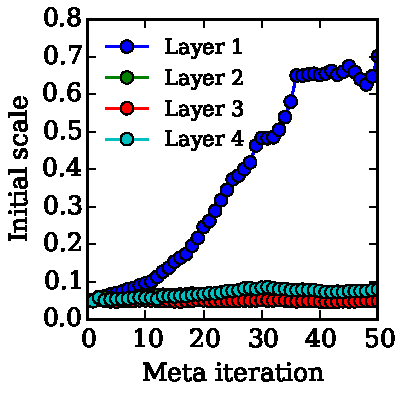
\includegraphics[width=0.5\columnwidth, height=0.5\columnwidth]{../experiments/Feb_3_training_schedules/3_adam_50/init_bias_learning_curve.pdf} &
\hspace{-1em}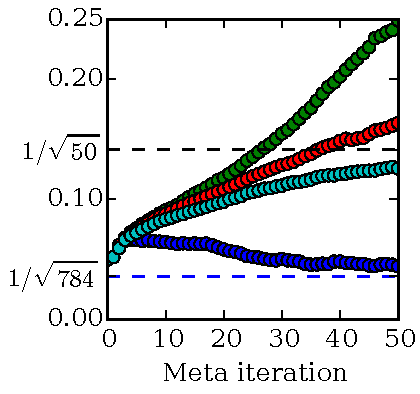
\includegraphics[width=0.5\columnwidth, height=0.5\columnwidth]{../experiments/Feb_3_training_schedules/3_adam_50/init_weight_learning_curve.pdf}
\end{tabular}
\end{center}}

\frame[plain]{\frametitle{Optimizing training data} 
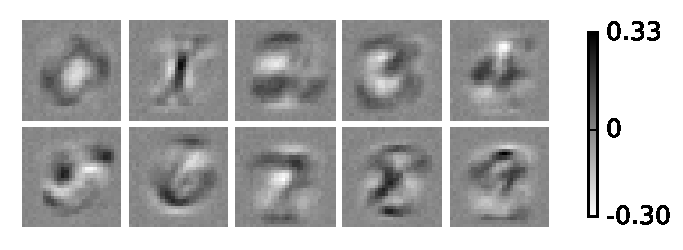
\includegraphics[width=\columnwidth]{../experiments/Jan_19_optimize_data/9_color_bar/fake_data.pdf}} 

\frame[plain]{\frametitle{Optimizing neural network architectures}
\begin{itemize} 
  \item Architecture is regularization
  \item Regularization can be continuous
  \item Continuous functions can be differentiated
  \item Consider: convnets, recurrent nets, multitask nets, ...
\end{itemize}}

\frame[plain]{\frametitle{Optimizing regularization: polyglot}
\begin{center}
\begin{tabular}{cc}
\hspace{-3mm}\rotatebox{90}{\qquad Rotated \qquad \quad Original} & 
\hspace{-3mm}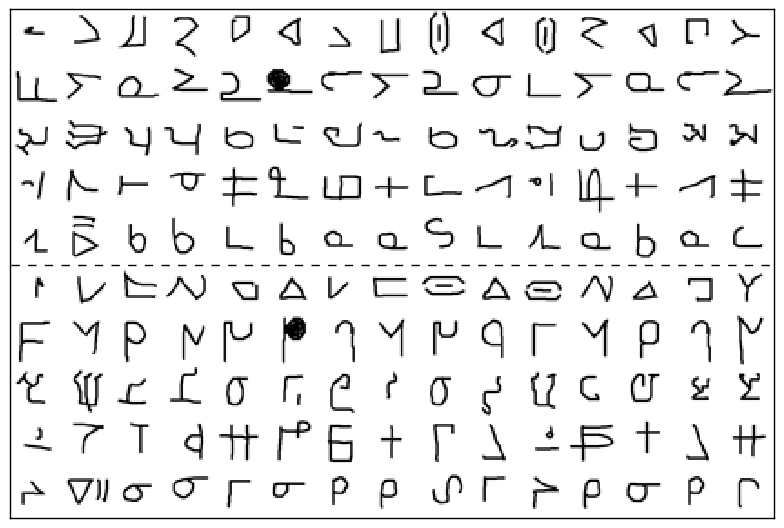
\includegraphics[width=0.85\columnwidth]{../experiments/Feb_4_augmented_omniglot/2_rotated_90/all_alphabets.png}
\end{tabular}
\end{center}}

\newcommand{\omniimagea}[2]{\parbox{4em}{\includegraphics[width=1.4cm]{../experiments/Feb_4_augmented_omniglot/2_rotated_90/minifigs/learned_corr_#1_#2.pdf}}}%
\newcommand{\omniimageb}[1]{\omniimagea{#1}{0} & \omniimagea{#1}{1} & \omniimagea{#1}{2}}%

\frame[plain]{\frametitle{Optimizing regularization: Omniglot}
\begin{center}
\begin{tabular}{c@{\hskip 0.9em}ccc@{\hskip 0.9em}c@{\hskip 0.9em}c}%
\renewcommand{\tabcolsep}{1pt}
& Input   & Middle  & Output & Train & Test\\
& weights & weights & weights & error & error \\
\parbox{3.7em}{Separate networks} & \omniimageb{no_sharing}      & 0.61 & 1.34\\ \hline
\parbox{3.7em}{Tied weights}      & \omniimageb{full_sharing}    & 0.90 & 1.25\\ \hline
\parbox{3.7em}{Learned sharing}   & \omniimageb{learned_sharing} & 0.60 & \bf 1.13
\end{tabular}
\end{center}}

\frame[plain]{\frametitle{Limitations: Chaotic learning dynamics}
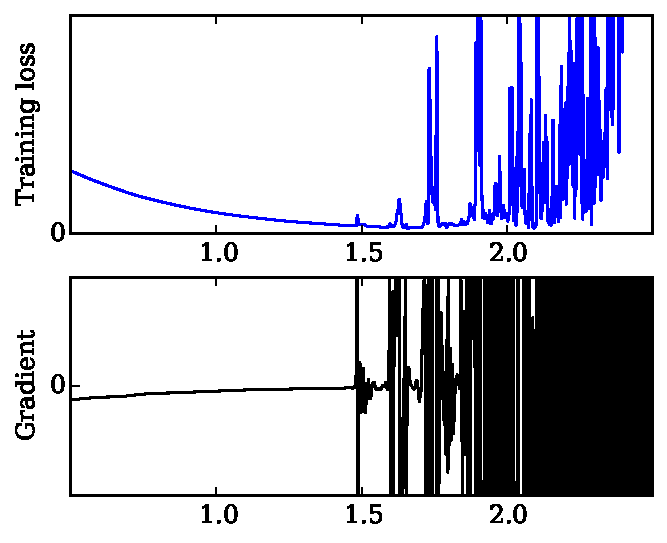
\includegraphics[width=0.9\columnwidth]{../experiments/Jan_14_learning_rate_wiggliness/3/chaos.pdf}
\vspace{-1.6em}
\center Learning rate}

%% \frame[plain]{\frametitle{Other possible applications}} % DM

\frame[plain]{\frametitle{Technical Challenge: Memory}
\begin{itemize}
\item Need access to entire learning trajectory
\item Only require LIFO access
\item Could we recompute the learning trajectory in reverse?
\end{itemize}}

\frame[plain]{\frametitle{SGD (with momentum) is Reversible}
Forward update rule:
\begin{align*}
\vx_{t+1} & \leftarrow \vx_t + \alpha \vv_t \\
\vv_{t+1} & \leftarrow \beta \vv_t - \nabla L\left(\vx_{t+1}\right)
\end{align*}
Reverse update rule:
\begin{align*}
\vv_{t} & \leftarrow \left(\vv_{t+1} + \nabla L\left(\vx_{t+1}\right)\right)/\beta \\
\vx_{t} & \leftarrow \vx_{t+1} - \alpha \vv_t
\end{align*}
}

\frame[plain]{\frametitle{Naive reversal \phantom{... Fails!}}
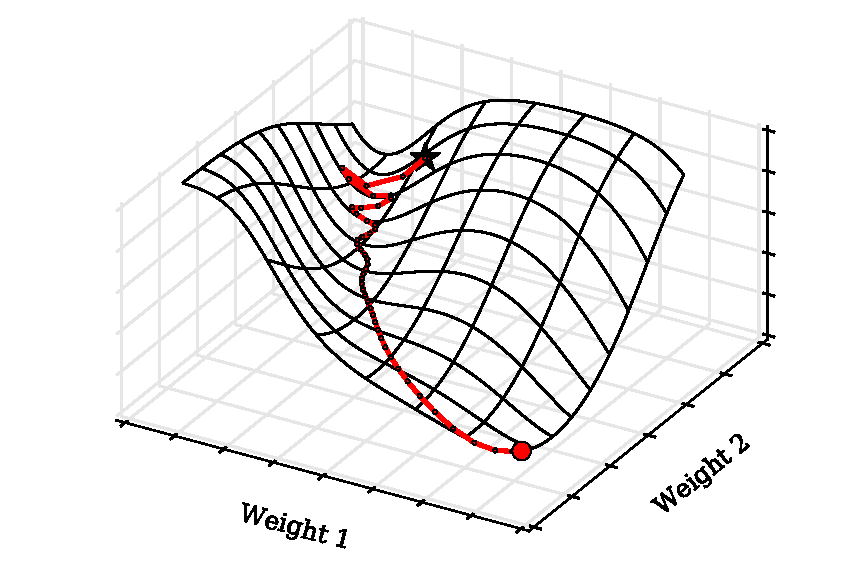
\includegraphics[width=0.9\columnwidth]{../experiments/Jan_25_Figure_1/4_naive_reverse/learning_curve_forward.pdf}}

\frame[plain]{\frametitle{Naive reversal ... Fails!}
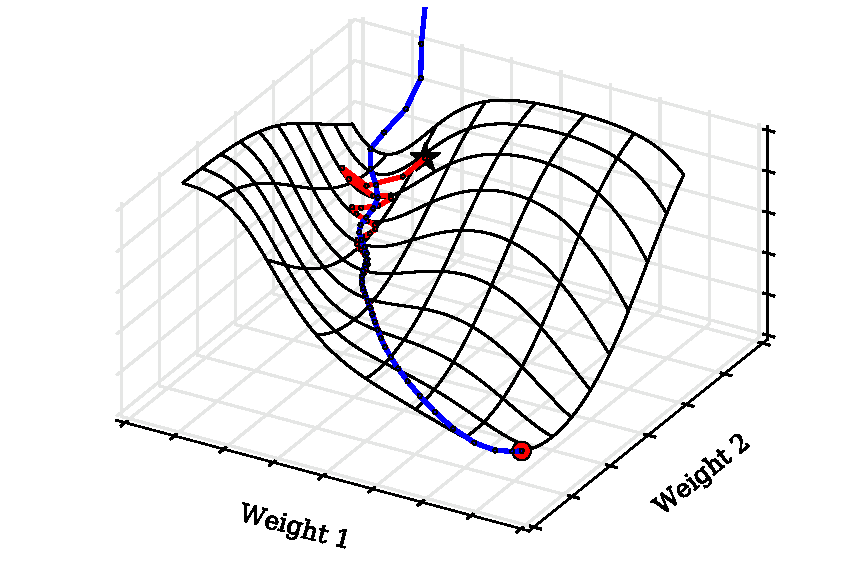
\includegraphics[width=0.9\columnwidth]{../experiments/Jan_25_Figure_1/4_naive_reverse/learning_curve_reverse.pdf}}

\frame[plain]{\frametitle{A closer look as reverse SGD}
Forward update rule:
\begin{align*}
\vx_{t+1} & \leftarrow \vx_t + \alpha \vv_t \\
\vv_{t+1} & \leftarrow \beta \vv_t - \nabla L\left(\vx_{t+1}\right)
\end{align*}
Reverse update rule:
\begin{align*}
\vv_{t} & \leftarrow \left(\vv_{t+1} + \nabla L\left(\vx_{t+1}\right)\right)/\beta \\
\vx_{t} & \leftarrow \vx_{t+1} - \alpha \vv_t
\end{align*}
\pause
\begin{itemize}
\item We destroy $\log\beta$ nats of entropy per parameter per iteration 
\item Can we set $\beta = 1$?
\pause
\item No! We require $\beta < 1$ for optimization to converge
\end{itemize}}

\frame[plain]{\frametitle{Entropy and Optimization are Deeply Connected}
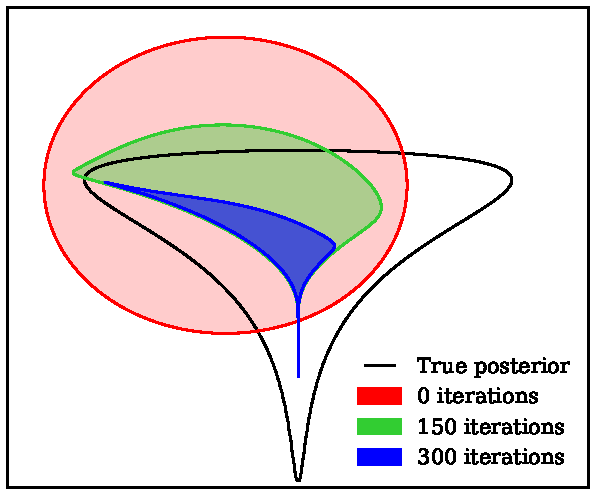
\includegraphics[width=0.9\columnwidth]{talkfigs/dists}}

\frame[plain]{\frametitle{Storing the entropy efficiently}
\begin{itemize} 
\item How can we store the $\log_2\beta$ bits upon multiplication?
\pause
\item Express $\beta$ as a rational number and push/pop remainders from an information buffer
\item Information buffer can use any LIFO coding method
\item $\sim$200X memory savings ($\beta \sim 0.9$)
\end{itemize}
Example code:

\lstset{basicstyle=\small\ttfamily\bfseries}
\lstinputlisting{code/infobuffer.py}}
\frame[plain]{\frametitle{Summary}
\begin{itemize}
\item We can compute gradients of learning procedures
\item This lets us do meta-learning
\item There is a deep connection between learning and entropy
\end{itemize}}

\end{document}
